\documentclass[10pt, letterpaper]{article}
        \usepackage[utf8]{inputenc}
        \usepackage[margin=1in]{geometry}
        \usepackage{fancyhdr}
        \usepackage{titling}
        \usepackage{enumitem}
        \usepackage{mathtools}
        \usepackage{amssymb}
        \usepackage{xfrac}
        \usepackage{booktabs}
        \usepackage{graphicx}
        \usepackage{wrapfig, blindtext}
        \usepackage{hyperref}
        \usepackage{enumerate}
        \usepackage{multicol}
        
        

        
        \setlength{\parindent}{0pt}

\title{Journal 2}
        \author{Sudhan Chitgopkar}
        \date{\today}
        
        % headers -- no need to change
        \pagestyle{fancy}
        \fancyhf{}
        \lhead{SPECPOL}
        \chead{UGAMUNC XXVII}
        \rhead{\thedate}

\begin{document}

Welcome to UGAMUNC XXVII! My name is Julia O'Neal, and I am so excited
to chair the 6th session of the Special Political and Decolonization
Committee with my co-chair, Joshua Walker. UGAMUNC is a conference that
I have a deep passion and appreciation for, as I have been attending it
since I was a freshman in high school. Now, as a first-year at the
University of Georgia, I hope to do it justice as we work with you to
have a successful weekend! \\

I am from Roswell, Georgia and am currently studying in the School of
Public and International Affairs for a degree in international affairs
with a French minor. I have been passionately involved in Model UN for 7
years, as well as the Sustainable Development Goals Club, the Swiss
exchange program, and my school's film program. In my free time, I paint
surrealist portraits, volunteer as a tech assistant at my local church,
work with kids, and spend time with my friends, family, and four cats. \\

I would also like to introduce you to Joshua Walker, our incredible
co-chair. He is a second-year double major in international affairs and
economics with a French minor. He is involved in the Roosevelt
Institute, the Economics Society, Campus Kitchen, and the American
Society of Law, Medicine and Ethics. In his free time, he loves cooking,
baking, reading, and hanging with friends at various Athenian coffee
shops. This is his first year in Model UN, and he is excited to get
involved! \\

In this conference, we ask that you work with us to ensure the safety
and sanctity of your peers. COVID-19 has brought unprecedented change to
every aspect of our lives, but we hope to provide normalcy and
enrichment by continuing UGAMUNC, as modified as it may need to be to
ensure the health of our delegates, faculty, and staff. \\

As a delegate in our committee, we expect that you will compete to the
best of your ability and prepare adequately. With this said, we also
would like to address that this committee will at times discuss
politically sensitive topics. Thus, we expect that you will compete with
the highest level of professionalism and debate responsibly.
Additionally, as delegates of your country, we expect that the scope of
your position papers and your proposed strategies in debate are in line
with the views of your country. Delegates should consider the history,
politics, culture, and demographics of the country which they represent.
Even if you do not personally agree with these views, the work of
SPECPOL is meant to put forth resolutions for each country and address
problems facing the international community; therefore, it is imperative
that each country is represented in its true form. \\

Please contact me with any questions you might have at my email provided
below. Finally, please submit your completed position papers to me and
Joshua by 11:59 PM on February 1st. We wish you the best of luck! \\

Julia O'Neal and Joshua Walker

\texttt{\href{mailto:Julia.oneal@uga.edu}{{Julia.oneal@uga.edu}}},
\texttt{\href{mailto:jbw01332@uga.edu}{{jbw01332@uga.edu}}}

\newpage
\tableofcontents
\newpage
\section{Background}

The Special Political and Decolonization Committee (SPECPOL) is the
fourth General Assembly Committee of the United Nations. Originally, the
fourth committee was solely responsible for decolonization and
trusteeship issues. In 1945, there were 750 million people living under
colonial power in either Trust Territories or non-self-governing
territories. Due to the work of the committee, there are now only 2
million people living under these conditions, and all eleven
UN-designated trusteeship territories have become
independent.\footnote{``Decolonization.'' Accessed October 31, 2020.
  https://www.un.org/en/sections/issues-depth/decolonization/.} Because
of the severe decline of decolonization issues, the fourth committee's
workload had severely decreased and merged with the Special Political
Committee in 1993. The Special Political Committee branched out from the
first committee, handling only certain political issues. It was briefly
turned into the seventh main general assembly committee before merging
with the fourth committee. \footnote{``United Nations General Assembly
  Fourth Committee.'' Wikipedia. Wikimedia Foundation, October 15, 2020.
  https://en.wikipedia.org/wiki/United\_Nations\_General\_Assembly\_Fourth\_Committee.}\\
  
The current SPECPOL committee is made of five Secretariat members, led
by Secretary Sangeeta Sharma. Since it is one of the GA committees,
every member nation participates and has one vote when voting on
resolutions. It provides a unique forum for political discourse in an
international, multilateral fashion.\footnote{``United Nations, Main
  Body, Main Organs, General Assembly.'' United Nations. United Nations.
  Accessed October 31, 2020. https://www.un.org/en/ga/fourth/.}\\
  
SPECPOL conducts the committee by annually considering a set of
continuous issues every assembly. The annual topic list includes five
decolonization related issues, the effects of atomic radiation, topics
on information, reviewing peacekeeping operations, United Nations Relief
and Works Agency for Palestinian Refugees in the Near East (UNRWA), the
Report of the Special Committee on Israeli Practices, and the peaceful
use of outer space.\footnote{``United Nations, Main Body, Main Organs,
  General Assembly.'' United Nations. United Nations. Accessed October
  31, 2020. https://www.un.org/en/ga/fourth/.} In conjunction with
reviewing peacekeeping operations, SPECPOL has a set of special
political missions that it reviews annually. Current missions include
the implementation of a peace and security framework in the Democratic
Republic of Congo and the Region, the United Nations Assistance Mission
in Somalia to stabilize domestic election processes, and the mission in
Columbia to build stable and lasting peace.\footnote{United Nations
  Peacekeeping Operations, Special Political Missions and Other
  Political Presences. Accessed October 31, 2020.
  https://www.unmissions.org/.}\\
  
This committee has played a vital role in the international system by
focusing on very specific issues that have been overlooked in more broad
international committees. Additionally, by annually revisiting the same
issues, SPECPOL ensures continuous attention and policy development on
issues such as the human rights of Palestinians and economics in
non-governing territories. The special political missions also serve a
vital role in focusing continued international support for very
particular issues such as those in Syria, Myanmar, or Western Sahara.
Without the continued focus by the UN, some of these issues would not
gain as much international attention.

\newpage
\section{Topic A: Consideration of Ethical Uses of Space in Advancing Society}

\subsection{Introduction}

Space law is unlike that of Earth. While the governing laws of the
international system of Earth are designed for purposes directly
regarding preserving humanity and sovereignty, space has an entirely
different set of requirements. The priority of space law is to promote
science and sustainability. International treaties have been set forth
forbidding certain behaviours in space, but the treaties are not
universally recognized. \\

Humanity is rapidly expanding at an unsustainable rate. For decades,
this growth has opened up conversations of increasingly more realistic
basis about the possibility of colonizing space and celestial bodies.
Science fiction popularized a vision of humanity living on other
planets, moons, or self-sustaining spaceships. However, current space
law forbids this. \\

As the Specific Political and Decolonization Committee, the issue of
reconsidering space law to account for human progress must be taken into
account with peace and political sustainability in mind. The committee
must address the possibility of loopholes that have emerged over time,
clauses that have evolved in relevancy, and enforcement for the greater
good of humanity. Rules regarding the proper use of space must be
considered with both the present and the future in mind, as well as
making sure solutions are ethical, sustainable, and fair. 

\subsection{History / Past UN Action}

The end of World War II began the infamous Space Race between the United
States and the Soviet Union. At the time, space travel was seen as a
symbol of power amongst the global superpowers, each wanting to prove
that their economic system could foster fruitful innovation. Competition
pushed progress and, within a decade, the Soviet Sputnik program put the
first man in space while the American Apollo program landed a man on the
moon.\footnote{``The Space Race.'' History.com. A\&E Television
  Networks, February 22, 2010.
  https://www.history.com/topics/cold-war/space-race.} After the 1696
moon landing, space travel became less urgent for public image, but
progress still ensued. The 1970s saw SkyLab, the American space station,
while the 1980s brought a surge of satellite cameras to give better
insight on our planet and others. The United States launched an
extremely successful 30-year space program, ending in 2011. Of the more
than 100 shuttle missions, only two were disastrous, killing 7 members
each. The International Space Station (ISS) is another milestone in
space exploration, specifically regarding cooperation and unification of
humanity. \\

One fundamental moment in the history of space law was the adoption of
the Outer Space Treaty, which sets out regulations for ethical and
sustainable use of space. Formally known as the Treaty on Principles
Governing the Activities of States in the Exploration and Use of Outer
Space, including the Moon and Other Celestial Bodies, it is commonly
referred to as the OST. It went through the process of drafting,
adoption, and ratification throughout the 1960s.\footnote{Wickramatunga,
  Robert. ``United NationsOffice for Outer Space Affairs.'' Accessed
  October 21, 2020.
  https://www.unoosa.org/oosa/en/ourwork/spacelaw/treaties/introouterspacetreaty.html.}
It has been ratified by 110 states, with another 23 that have signed
without ratification. \\

Some defining parts of the OST are its emphasis on peace, cooperation,
sustainability, and responsibility. It emphasizes that the use of space
must be universally beneficial to all mankind. Space is without
sovereignty. It should not be colonized, polluted, or weaponized with
weapons of mass destruction. Countries are responsible for any actions
taken in space and are consequently responsible for any damage
done.\footnote{Wickramatunga, Robert. ``United NationsOffice for Outer
  Space Affairs.'' Outer Space Treaty. Accessed October 21, 2020.
  https://www.unoosa.org/oosa/en/ourwork/spacelaw/treaties/outerspacetreaty.html.} 

\subsection{International Involvement}

The topic of space exploration is more relevant to some countries than
others. The top 10 countries with large space programs are the United
States, China, Russia, Japan, the United Kingdom, India, Canada,
Germany, France, and Luxembourg.\footnote{Admin. ``Verdict Media
  Limited.'' Aerospace Technology, January 23, 2020.
  https://www.aerospace-technology.com/features/featurethe-10-countries-most-active-in-space-4744018/.}
The inserted graph shows prevalence, ownership, and usage of
satellites.\footnote{Chatham House. ``Why We Need a New Global Code of
  Conduct for Outer Space.'' World Economic Forum, September 11, 2019.
  https://www.weforum.org/agenda/2019/09/why-we-need-a-global-code-of-conduct-for-outer-space/.}

However, many other countries have their own space programmes or are
members of larger ones. There are about 40 space agencies globally, with
some countries having multiple agencies, such as China or the Republic
of Korea, and some agencies having multiple countries, such as the
European Space Agency (ESA) or the Asia Pacific Space Cooperation
Organization (APSCO). \footnote{Wickramatunga, Robert. ``United
  NationsOffice for Outer Space Affairs.'' World Space Agencies webpage.
  Accessed October 21, 2020.
  https://www.unoosa.org/oosa/en/ourwork/space-agencies.html.}\\
  
\begin{wrapfigure} {r} {0pt}
\centering
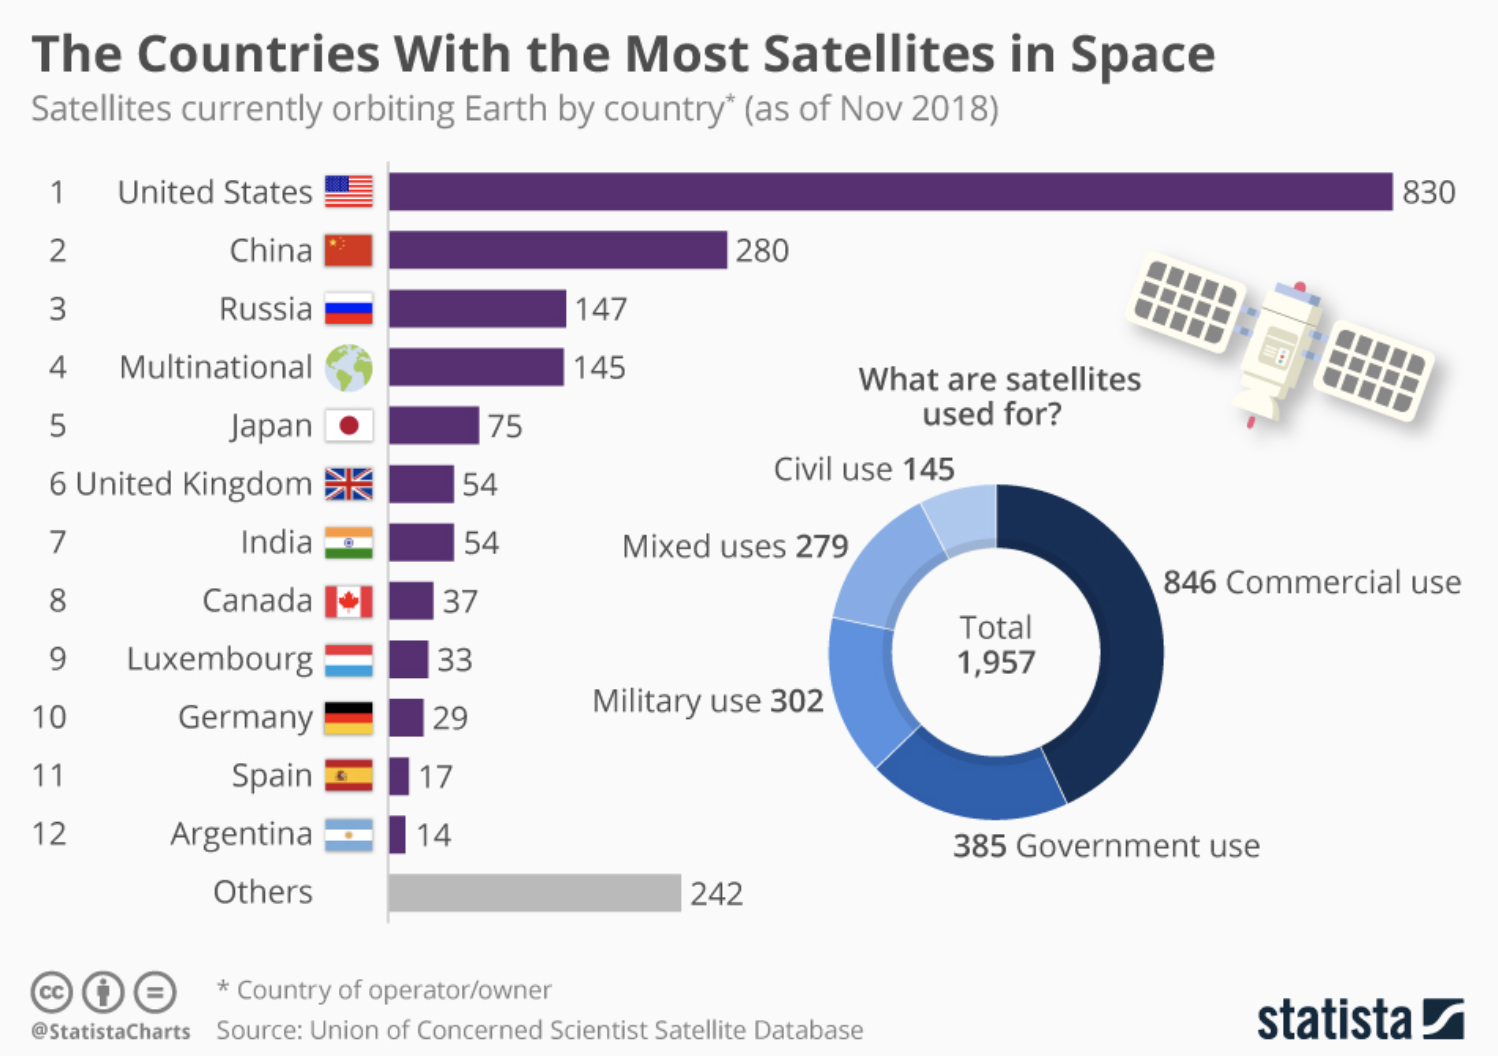
\includegraphics[scale = 0.35]{image3.png} 
\end{wrapfigure}

However, exploration and theoretical colonization is not the extent of
progress. The discussion of the ethical use of space is a discussion
affecting the entire international system. Although not all countries
have the means to conduct their own space research, most countries
benefit from space research in the form of satellite imagery, Global
Positioning Systems, and satellite phones. \\

The International Space Station shows a successful example of multiple
countries being involved in one singular collaborative space mission.
Since 2000, the orbiting space base has had occupants from 17 different
countries. The international cooperation seen in the development and
usage of the ISS could potentially be a framework for future
collaborative space endeavors. \\

Certain parts of the OST leave questions of whether the document should
be revisited. The document specifies that all celestial bodies cannot be
used or occupied by any state. While this is not a pressing issue, the
concept of colonizing celestial bodies may become an eventual concern
and may need to be revisited. The OST also specifies that any action
taken in space must have a respective state, or several, which can be
held accountable for it. This particularly raises questions of non-state
actors who wish to use space and whether it should be allowed.
Additionally, the specification that prohibits weapons of mass
destruction (WMD) in space leaves loopholes. Intercontinental Ballistic
Missiles (ICBMs) travel through lower levels of outer space despite
being WMDs. \\
\newpage
\subsection{Vocabulary}

\begin{itemize}
\item 
\textbf{Outer Space Treaty (OST)}: a treaty commonly linked to the
historical Antarctic Treaty in that it sought to prevent new forms of
colonialism, specifically in outer space, while also preventing
expansion-related competition\footnote{``Outer Space Treaty.'' U.S.
  Department of State. U.S. Department of State. Accessed October 21,
  2020. https://2009-2017.state.gov/t/isn/5181.htm.}

\item 
\textbf{Multinational Corporations (MNCs)}: a corporation which ``has
facilities and other assets in at least one country other than its home
country;'' often uses one country to host its headquarters\footnote{Chen,
  James. ``Multinational Corporation (MNC).'' Investopedia.
  Investopedia, August 28, 2020.
  https://www.investopedia.com/terms/m/multinationalcorporation.asp.}

\item 
\textbf{Intercontinental Ballistic Missiles (ICBMs)}: ``land-based,
nuclear-armed ballistic missile{[}s{]} with a range of more than 3,500
miles (5,600 km);''\footnote{Gregersen, Eric. ``ICBM.'' Encyclopædia
  Britannica. Encyclopædia Britannica, inc. Accessed October 21, 2020.
  https://www.britannica.com/technology/ICBM.} countries with ICBMs
include the United States, Russia, China, France, North Korea, the
United Kingdom and India\footnote{``Intercontinental Ballistic
  Missile.'' Wikipedia. Wikimedia Foundation, October 17, 2020.
  https://en.wikipedia.org/wiki/Intercontinental\_ballistic\_missile.}

\item 
\textbf{Weapons of Mass Destruction (WMDs)}: as defined by U.S law: ``a
destructive device, such as an explosive or incendiary bomb, rocket, or
grenade; a weapon that is designed to cause death or serious injury
through toxic or poisonous chemicals; a weapon that contains a
biological agent or toxin; or a weapon that is designed to release
dangerous levels of radiation or radioactivity''\footnote{``WMD.'' FBI.
  FBI, May 3, 2016. https://www.fbi.gov/investigate/wmd.}
\end{itemize}

\subsection{Questions to Consider}

\begin{enumerate}
\def\labelenumi{\arabic{enumi}.}
\item
  
  Is it ethical to capitalize on resources from outer space, or should
  celestial bodies be preserved?
  
\item
  
  Should corporations, specifically MNCs be allowed to conduct
  activities in space without direct approval of a singular state?
  
\item
  
  How heavily should space law be enforced, and what stops a global
  superpower from theoretically ignoring regulations and claiming a
  celestial body?
  
\item
  
  How can the committee define the gray area of ``for the good of
  mankind'' to properly enforce agreements involving use of space?
  
\item
  
  Is it ethical to send humans into potentially unsafe situations in
  space if it is for scientific benefit? What about animals?
  
\item
  
  Considering extensive travel time, would it be feasible to explore
  Mars and potentially other celestial bodies when occupation of it is
  forbidden? Would temporary visits make the effort worth the time it
  takes?
  
\item
  
  If non-state actors such as MNCs were to be allowed to pursue space
  exploration, how would monopolization of potential space industries be
  stopped?
  
\item
  
  If non-state actors were to be allowed to pursue space exploration
  when advancements and technology for it become more easily accessible,
  what stops potential terrorist groups from utilizing space?
  
\item
  
  How should space junk such as dead satellites be regulated?
  
\end{enumerate}

\subsection{Further Reading}

\begin{enumerate}
\def\labelenumi{\arabic{enumi}.}
\item
  
  \texttt{{\href{https://spacepolicyonline.com/topics/space-law/}{Space
  Law}}}
  
\item
  
 \texttt{{\href{https://www.un.org/press/en/2009/gaspd433.doc.htm}{Debating
  Outer Space Cooperation, Fourth Committee Hears Growing Number of
  Actors in Outer Space Could Risk Security of Space Assets, Limit Scope
  of Peaceful Uses Meetings Coverage and Press Releases}}}
  
\item
  
  \texttt{{\href{https://www.un.org/press/en/2019/gaspd705.doc.htm}{Fourth
  Committee Approves Draft Resolution on Peaceful Uses of Outer Space,
  as Delegates Conclude General Debate \textbar{} Meetings Coverage and
  Press Releases}}}
  
\item
  
  \texttt{{\href{https://www.nasa.gov/sites/default/files/files/Benefits-Stemming-from-Space-Exploration-2013-TAGGED.pdf}{Benefits
  Stemming from Space Exploration}}}
  
\item
  
  \texttt{{\href{https://www.nhm.ac.uk/discover/what-is-space-junk-and-why-is-it-a-problem.html}{What
  is space junk and why is it a problem?}}}
  
\end{enumerate}

\newpage
\section{Topic B: Maintaining Peace in the Kurdish Region}

The Kurds are an ethnic-linguistic group of people who originated from
the Zagros mountains in the Middle East. Today, their population
(estimated at 25 million to 30 million) has spread out across much of
the Middle East and makes up a large portion of their population. They
are the fourth largest ethnic group in the Middle East. \\

Because of their unique origin, the Kurds have proposed the formation of
the State of Kurdistan (shown in image\footnote{``Who Are the Kurds?''
  BBC News. BBC, October 15, 2019.
  https://www.bbc.com/news/world-middle-east-29702440.}), which
translates to ``Land of the Kurds''. The proposed state rides the border
between Turkey, Syria, Iraq, Iran, and Armenia, where the majority of
the Kurdish population lives. The majority of the land lies in Turkey.
This state is theoretical, seeing as the sovereignty for the land it
requires belongs to the five respective countries. As the Special
Political and Decolonization Committee, the mandate specifies
peacekeeping and decolonization as two of the issues SPECPOL is
responsible for, both of which apply to the issue of peace in the
Kurdish region. \\

\subsection{History} 

Although their exact ethnic origins are unknown, the Kurdish people can
be traced back to the Kurdish region for thousands of years. They
primarily lived as nomads, herding animals in the Zagros region and
Mesopotamian plains. They are primarily Sunni Muslims, although not
exclusively. Their language originates from Persian and Pashto as a
group of dialects. They have largely remained apolitical in terms of the
international system: the Kurds have never had an established state for
themselves, despite having organized into tribes and dynasties.
Sheikh-led tribes were common for a while, but eventually, the Kurds
integrated into society and lost their tribal structure.\footnote{Tikkanen,
  Amy. ``Kurd.'' Encyclopædia Britannica. Encyclopædia Britannica, inc.
  Accessed October 21, 2020. https://www.britannica.com/topic/Kurd.} \\

After World War 1, the Kurdish nationalist movement began to take root.
Despite never having a solidified state, the promise of one sparked
interest when The Treaty of Sèvres was signed in 1920. Supported by one
of US President Woodrow Wilson's 14 points, it recognized the formation
of Kurdistan, among other Arab states. Unfortunately for the Kurds, this
treaty was left unratified and soon after, it was overwritten by the
1923 Treaty of Lausanne. \\

The awarding and immediate revocation of recognition was a shock to the
Kurdish people. It sparked a movement of nationalism in the Kurdish
people, specifically the Kurds in the designated region, which has
continued on to the present day. They have consistently advocated for
the creation of their own state so that they're no longer a stateless
minority group, but they have not had any success.\footnote{``Kurdistan.''
  Encyclopædia Britannica. Encyclopædia Britannica, inc. Accessed
  October 21, 2020. https://www.britannica.com/place/Kurdistan.} Their
continuous desire for their own state stems largely from their strong
ethnic nationalism. The Kurds feel a stronger sense of nationalism in
their ethnic identity than in their national identity, which provides a
basis for a possible case for statehood. \\

Not all Kurds pursue the formation of Kurdistan in the same manner. The
Kurdish Workers Party (PKK) is a group of Kurdish nationalist extremists
who are recognized as a terrorist group by Turkey. Their presence in the
Middle East is a threat to international security and peace in the
region. From July 2015 to October 2020, over 5000 people have been
killed as a result of their violence.\footnote{``Turkey's PKK Conflict:
  A Visual Explainer.'' Crisis Group, October 9, 2020.
  https://www.crisisgroup.org/content/turkeys-pkk-conflict-visual-explainer.}
Amongst the desires of the peaceful Kurds, the presence of the PKK must
also be addressed by the committee. \\

\subsection{International Community / UN Involvement}

The majority of UN involvement in the Kurdish region has been focused on
human rights, de-escalation of conflict, and humanitarian aid. However,
in 2017, the UN Security Council voted against a referendum to establish
independence for Iraqi Kurds. The member states cited their reasons for
being that the referendum would be ``destabilizing,'' especially in the
fight against terrorist group ISIL, which the Kurdish forces have been
instrumental in. The goal is to postpone the referendum until a better
time.\footnote{Wires, News. ``UN Security Council Opposes Kurdish
  Independence Vote.'' France 24. France 24, September 22, 2017.} \\

Turkey is the sovereign nation most affected by the issue of Kurdish
independence. 20\% of Turkey is made of Kurds, and half of the Kurds are
Turkish. It largely denies the issue and does not fully recognize their
presence and unity. They are referred to as ``mountain Turks'' and their
language and culture are repressed.\footnote{The Kurds in Turkey.
  Accessed October 21, 2020.
  https://fas.org/asmp/profiles/turkey\_background\_kurds.htm.} \\

Other countries involved respond differently. Egypt is a large supporter
of the Kurdish independence movement. Iraq, in 2005, awarded the Kurds
an autonomous zone. It has self- governing powers but the 2017 vote for
independence was incomplete. \\

\subsection{Vocabulary}

\begin{itemize}
    \item 
\textbf{Nation}: A group of individuals who share similar values,
cultural aspects, and history\footnote{``Nations and States.''
  SparkNotes. SparkNotes. Accessed October 17, 2020.
  https://www.sparknotes.com/us-government-and-politics/political-science/nations-and-states/section1/.}
    \item 
\textbf{State}: An organized political unit under one
\href{https://en.wikipedia.org/wiki/Government}{government}, expressing
the value of sovereignty over political, economic, and legal
function\footnote{Duignan, Brian. ``State.'' Encyclopædia Britannica.
  Encyclopædia Britannica, inc. Accessed October 17, 2020.
  https://www.britannica.com/topic/state-sovereign-political-entity.}
    \item 
\textbf{PKK}: Partiya Karkerên Kurdistanê: Kurdistan Workers' Party, an
organization based in Turkey and Iraqi Kurdistan engaged in armed
conflict with the Turkish state for self-determination for the
Kurds\footnote{``PKK Definition and Meaning: Collins English
  Dictionary.'' PKK definition and meaning \textbar{} Collins English
  Dictionary. HarperCollins Publishers Ltd. Accessed October 21, 2020.
  https://www.collinsdictionary.com/us/dictionary/english/pkk.}
    \item 
\textbf{Sunni Muslim}: A member of the branch of Islam that accepts the
first four caliphs as rightful successors to Muhammad\footnote{``Sunni
  Muslim.'' Vocabulary.com. Accessed October 21, 2020.
  https://www.vocabulary.com/dictionary/Sunni Muslim.}
\end{itemize}

\subsection{{Questions to Consider}}

\begin{enumerate}
\item
  
  What constitutes having a right to statehood?
  
\item
  
  If Kurdistan were to officially form, how would the Kurds obtain the
  land from other states?
  
\item
  
  If Kurdistan were to officially form, what would happen to the
  non-Kurdish people in potential Kurdish territory who identify
  strongly with the state they are currently in?
  
\item
  
  How can the committee appeal to the interests of the Kurdish people
  while not entertaining the PKK?
  
\item
  
  How does the conflict for Kurdistan compare to other conflicts of
  nationalist boundaries, such as Palestine or Kashmir?
  
\end{enumerate}
\newpage
\subsection{Further Reading}

\begin{enumerate}
\def\labelenumi{\arabic{enumi}.}
\item
  
  \texttt{{\href{https://www.cia.gov/library/readingroom/docs/DOC_0000469140.pdf}{(ESTIMATED
  PUB DATE) THE KURDS: RISING EXPECTATIONS, OLD FRUSTRATIONS}}}
  
\item
  
  \texttt{\href{https://www.cia.gov/library/readingroom/docs/CIA-RDP79-00927A004100020004-3.pdf}{{KURDISH
  NATIONALISM IN THE MIDDLE EAST}}}
  
\item
  
  \texttt{{\href{https://www.globalsecurity.org/military/world/war/kurdistan-iran.htm}{Kurdistan
  - Iran}}}
  
\item
  
  \texttt{\href{https://www.middleeastmonitor.com/20150818-the-oppression-of-the-kurds-and-possible-solutions/}{{The
  oppression of the Kurds and possible solutions}}}
  
\end{enumerate}

\newpage
\section{Topic C: Hong Kong's Sovereignty and Global Involvement}

\subsection{Introduction}

The United Nations, from its mid-20th-century beginnings, has always
valued the principle of self-determination. One of its many tools for
ensuring that the population of the world gains access to this simple
right is the fourth General Assembly, a body that, by its most
fundamental definition, strives to ``decolonize'' those who desire
political participation and self-determination. Unfortunately, the
concept of decolonization has become even more difficult to apply in the
21st century, and one of the starkest examples of these complications is
the historically-charged case of Hong Kong. \\

The polity's past is riddled with colonialist intervention, state
handovers, and a historically unique political situation. Being under a
``one country, two systems'' framework, Hong Kong is meant to have
expansive self-determinism. However, recent events have led many in Hong
Kong to believe that their legally-protected rights are being brushed
aside by the Chinese government, and, with Hong Kong being an
international trading power (ranked 8th in the world in foreign
trade\footnote{Cheung, Tai Ming. "10. HONG KONG'S STRATEGIC IMPORTANCE
  UNDER CHINESE SOVEREIGNTY." (1998).}), the issue is hardly a regional
one. Protesters have been demanding reclamation of their protected
rights for well over a year, so this particular situation seems to be
one that should be addressed by the global community. \\

The goal of this body will be to thoroughly unpack the issues of alleged
Chinese intervention in what should be a mostly-autonomous political
unit, as well as discussing the general issues of 21st-century
self-determinism and the responsibilities of involved/uninvolved actors
in addressing it. \\

\subsection{History of Hong Kong}
  \begin{wrapfigure} {r} {0pt}
\centering
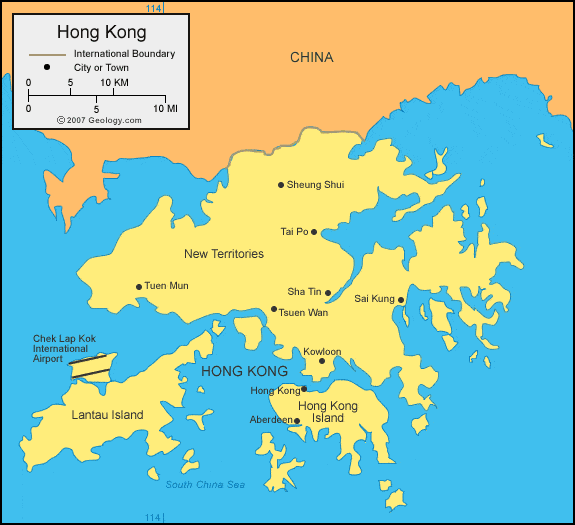
\includegraphics[scale = 0.35]{image4.png} 
\end{wrapfigure}

Hong Kong's past has featured a unique blend of war, drugs, colonialism,
and sub-state autonomous rule. The region's beginnings opened within the
setting of 3rd-century B.C. east Asian imperialism when, under the Qin
Dynasty, the area came under Chinese rule. The First Opium War between
the British and Chinese Empires in the mid-1800s, however, ceded Hong
Kong Island (the southernmost portion of the region) to Great Britain
through the Treaty of Nanjing. With its ideal geographic situation,
being bordered by both the South China Sea and China, Great Britain
began to desire greater regional control, sparking the Second Opium War.
Through the Convention of Beijing in 1860 and the Second Convention of
Peking in 1898, the modern boundaries of Hong Kong were set and the
region was now totally controlled by the British Empire\footnote{Little,
  Becky. ``How Hong Kong Came Under 'One Country, Two Systems' Rule,''
  September 3, 2019.
  https://www.history.com/news/hong-kong-china-great-britain.}.\\
  
According to the agreements between China and Great Britain, however,
Hong Kong was scheduled to be returned to China on July 1, 1997 (99
years after the Second Convention of Peking). Between 1898 and 1997, the
only disruption to British control of Hong Kong came during World War II
when Japan controlled much of Southeast Asia. However, Great Britain
maintained its presence, and in 1982, leaders from both China and the
U.K. met to discuss the transition set to incur in 15 years\footnote{Little,
  Becky. ``How Hong Kong Came Under 'One Country, Two Systems' Rule,''
  September 3, 2019.
  https://www.history.com/news/hong-kong-china-great-britain.}.
(image)\footnote{``Hong Kong Map and Satellite Image.'' geology.
  Accessed October 17, 2020.
  https://geology.com/world/hong-kong-satellite-image.shtml.}\\

In 1984, the Sino-British Joint Declaration was signed, outlining the
terms and stipulations of the transition, as well as a plan for
post-transition Hong Kong and its political/economic institutions and
ties with China. The declaration allowed Hong Kong to maintain its
current autonomy and its social, legal, judicial, and economic systems,
until 2047. In essence, the region was to ``remain unchanged for 50
years,'' per the agreement. This meant that Hong Kong could continue its
capitalist lifestyle while reaffirming the existing rights of speech,
religion, press, and assembly. Under this ``one country, two systems''
rule, Hong Kong became a Special Administrative Region with full
autonomy under China\footnote{Cheung, Gary. ``What Is the Sino-British
  Joint Declaration?'' South China Morning Post, July 4, 2019.
  https://www.scmp.com/news/hong-kong/politics/article/3017318/explainer-what-sino-british-joint-declaration-and-what-does.}.
The largest change was that China now had the power to appoint Hong
Kong's executive; however, it claimed it would do so in accordance with
the region's democratic election results\footnote{``Some Facts about the
  Basic Law.'' Some Facts about the Basic Law - index.html. Accessed
  October 17, 2020. https://www.basiclaw.gov.hk/en/facts/index.html.}.\\

The first hints at China's unwillingness to fully adhere to the deal
came in the early 2010s when Chinese leaders began affirming to British
diplomats that the U.K. had no authority to regulate China's abidance to
the agreement. In fact, the Chinese ambassador to Great Britain, Ni
Jian, even claimed that the Sino-British Joint Declaration was ``now
void and covered only the period from the signing in 1984 until the
handover in 1997.''\\

Protests have since sprung from Chinese intervention in Hong Kong's
domestic affairs, affairs that were supposedly protected under the joint
declaration. For example, in August 2014, the Chinese government
reformed the stipulations of Hong Kong's electorate system of universal
suffrage, now only allowing two or three candidates that are vetted by a
committee of ``pro-Beijing elites'' to run for the executive.
Essentially, China was now getting directly involved in Hong Kong's
democratic process, and the result was mass protests called the Umbrella
Revolution\footnote{Kaiman, Jonathan. ``Hong Kong's Umbrella Revolution
  - the Guardian Briefing.'' The Guardian. Guardian News and Media,
  September 30, 2014.
  https://www.theguardian.com/world/2014/sep/30/-sp-hong-kong-umbrella-revolution-pro-democracy-protests.}.
Again, in 2016, protests were spurred throughout the region, this time
in response to China's new verdict that executive candidates who
supported Hong Kong independence were no longer allowed to
run\footnote{Staff, TIME. ``Hong Kong Makes History With First
  Pro-Independence Rally.'' Time. Time, August 5, 2016.
  https://time.com/4440708/hong-kong-independence-china-localist/.}\footnote{Iyengar,
  Rishi. ``Hong Kong: Pro-Independence Candidate Barred From
  Elections.'' Time. Time, August 3, 2016.
  https://time.com/4436253/hong-kong-election-briefing-protests-edward-leung-china-independence/.}.
In 2019, the Chinese government introduced an extradition bill that
would allow Hong Kong to extradite alleged criminals to China for trial.
Many claimed that this bill would expose those in Hong Kong to a flawed
Chinese judicial system, and after months of protests opposing its
implementation, the proposal was withdrawn\footnote{Li, Jeff. ``Hong
  Kong-China Extradition Plans Explained.'' BBC News. BBC, December 13,
  2019. https://www.bbc.com/news/world-asia-china-47810723.}.\\


Most recently, protestors lined the streets on China's National Day
(October 1st), 2020 in defiance of Chinese intervention in Hong Kong
affairs. Protestors were quickly shut down by police\footnote{Ramzy,
  Austin, Elaine Yu, and Tiffany May. ``On China's National Day, Hong
  Kong Police Quash Protests.'' The New York Times. The New York Times,
  October 1, 2020.
  https://www.nytimes.com/2020/10/01/world/asia/hong-kong-protests-china.html.}.
This comes only a few months after China passed a national security law
in June of 2020 that severely curtails Hong Kong citizens' rights to
free speech, imposing penalties on those that promote secession,
undermining the central government, terrorism, and foreign
collusion\footnote{Tsoi, Grace, and Lam Cho Wai. ``Hong Kong Security
  Law: What Is It and Is It Worrying?'' BBC News. BBC, June 30, 2020.
  https://www.bbc.com/news/world-asia-china-52765838.}.

\subsection{{Self Determination: History and Applications}}

Self-determination as a concept first took hold with the philosophical
writings of Immanuel Kant\footnote{Dryden, Jane. ``Autonomy.'' Internet
  Encyclopedia of Philosophy. Accessed October 17, 2020.
  https://iep.utm.edu/autonomy/.}. These ideas, in conjunction with
other notable philosophers (Rousseau, Locke, etc.), inspired colonies
and countries such as the United States and France to use the principle
of self-determination to overthrow the previously existing government
structure\footnote{Kolla, Edward. ``The French Revolutionary Origins of
  National Self-Determination -- Edward Kolla: Aeon Ideas.'' Aeon. Aeon,
  October 17, 2020.
  https://aeon.co/ideas/the-provocation-of-national-self-determination.}.
This created a wave of nationalism in the late-18th century and
early-19th century that fought against imperialist structures and spread
self-determinist values\footnote{McLean, John. ``History of Western
  Civilization II.'' Self-Determination and New States \textbar{}
  History of Western Civilization II. Accessed October 17, 2020.
  https://courses.lumenlearning.com/suny-hccc-worldhistory2/chapter/self-determination-and-new-states/.}.\\


The wave of nationalism gave way to a new imperialism; colonial powers
yet again began to carve up lesser developed countries and drain their
resources. After World War I and II, decolonization efforts took hold,
in part due to an international push for self-determination\footnote{cmvt.
  ``Reasons for the End of Imperialism, Decolonization and Emergence of
  New Nation-States and Its Impact,'' September 5, 2015.
  https://cmvtcivils.wordpress.com/2015/09/05/reasons-for-the-end-of-imperialism-decolonization-and-emergence-of-new-nation-states-and-its-impact/.}.
At the end of World War I, Woodrow Wilson's Fourteen Points detailed the
creation of a League of Nations that would execute ``a variety of
geographic arrangements carrying out the principle of
self-determination''\footnote{``Woodrow Wilson : Fourteen Points Speech
  (1918).'' U.S. Embassy \& Consulate in the Republic of Korea, February
  11, 2020.
  https://kr.usembassy.gov/education-culture/infopedia-usa/living-documents-american-history-democracy/woodrow-wilson-fourteen-points-speech-1918/.}.\\


The United Nations, the more successful international version of the
League, also made self-determination one of its foremost goals, even
cementing its importance into the UN charter\footnote{``Chapter I: UN
  Charter.'' United Nations. United Nations. Accessed October 17, 2020.
  https://www.un.org/en/sections/un-charter/chapter-i/index.html.}. As
one of its first actions, the UN signed a resolution subtitled
"Declaration on the Granting of Independence to Colonial Countries and
Peoples," which moved to immediately take steps to give governmental
power back to the people of Trusts and Non-Self-Governing
Territories\footnote{``Decolonization.'' United Nations. United Nations.
  Accessed October 17, 2020.
  https://www.un.org/en/sections/issues-depth/decolonization/index.html.}.\\


The UN has had mixed success in juggling the important values of both
self-determinism and sovereignty, and the increasingly contentious
relations between Hong Kong and China introduce a new, complex problem
for this committee to tackle.
\newpage
\subsection{Vocabulary}

\begin{itemize}
    \item 
\textbf{Extradition}: ``the removal of a person from a requested state
to a requesting state for criminal prosecution or
punishment''\footnote{``Extradition.'' Legal Information Institute.
  Legal Information Institute. Accessed October 17, 2020.
  https://www.law.cornell.edu/wex/extradition.}
    \item 

\textbf{Nation}: a group of individuals who share similar values,
cultural aspects, and history\footnote{``Nations and States.''
  SparkNotes. SparkNotes. Accessed October 17, 2020.
  https://www.sparknotes.com/us-government-and-politics/political-science/nations-and-states/section1/.}
    \item 

\textbf{``One country, two systems''}: China's current situation in
which Hong Kong is given the abilities and sovereignty of a Special
Administrative Region, maintaining basic autonomy, while still under
Chinese territory\footnote{Tam, Felix, and Clare Jim. ``\,'One Country,
  Two Systems' Can Continue beyond 2047: Hong Kong Leader.'' Reuters.
  Thomson Reuters, January 16, 2020.
  https://www.reuters.com/article/us-hongkong-protests/one-country-two-systems-can-continue-beyond-2047-hong-kong-leader-idUSKBN1ZF0NO.}
    \item 

\textbf{Self-determinism}: the right of a people to determine its own
destiny; a principle allowing a people to choose its own political
status and to determine its own form of economic, cultural, and social
development\footnote{``Self-Determination.'' UNPO, September 21, 2017.
  https://unpo.org/article/4957.}
    \item 

\textbf{Sino-British Joint Declaration}: an agreement made in 1982
between Great Britain and China outlining the transition of Hong Kong
from the British Empire to China, as well as Hong Kong's future autonomy
under the Chinese state\footnote{Cheung, Gary. ``What Is the
  Sino-British Joint Declaration?'' South China Morning Post, July 4,
  2019.
  https://www.scmp.com/news/hong-kong/politics/article/3017318/explainer-what-sino-british-joint-declaration-and-what-does.}
    \item 

\textbf{State}: an organized political unit under one
\href{https://en.wikipedia.org/wiki/Government}{government}, expressing
the value of sovereignty over political, economic, and legal
function\footnote{Duignan, Brian. ``State.'' Encyclopædia Britannica.
  Encyclopædia Britannica, inc. Accessed October 17, 2020.
  https://www.britannica.com/topic/state-sovereign-political-entity.}
\end{itemize}

\subsection{{Questions to Consider}}

\begin{enumerate}
\def\labelenumi{\arabic{enumi}.}
\item
  
  What is the best balance between self-determination and sovereignty;
  that is, at what point should the global community be allowed to
  intervene a state's sovereignty to help support self-determinist
  values?
  
\item
  
  In reviewing Hong Kong's politically complex past, what is the best
  way to proceed with the issue of growing Hong Kong discontent towards
  the Chinese government?
  
\item
  
  Are the recent protests really just a tool of the minority, while the
  majority of Hong Kong citizens are not unhappy with Chinese
  intervention? If so, what action is appropriate for the global
  community to take and what action would be an overstep?
  
\item
  
  Are violent police interventions in protests a violation of basic
  speech rights? Human rights? If so, how can countries urge China to
  discontinue such abusive and violent practices?
  
\item
  
  How should your country react, in recognition of recent events, to
  increasingly contentious Chinese-Hong Kong relations? What is your
  country's stance on the situation? Does it support intervention into
  Chinese affairs in order to establish/reestablish Hong Kong's
  autonomy?
  
\item
  
  Upon further evaluation and analysis of the Sino-British Joint
  Declaration, is China truly breaching this agreement? If so, should
  the U.K. be allowed to intervene within the role as a regulatory body
  of the agreement?
  
\item
  
  Broadly, is the ``one country, two systems'' approach a reasonable
  one? Was such an approach to Hong Kong's autonomy the best method of
  transitioning power from Great Britain to China, or was there a better
  solution?
  
\item
  
  Could the ``one country, two systems'' approach work elsewhere in the
  world where different nations vie for rights, representation, and
  power under one state (such as the case of many groups in Africa due
  to 18th/19th-century colonialism)?
  
\end{enumerate}

{\subsection{Suggested Reading}}

\begin{enumerate}
\def\labelenumi{\arabic{enumi}.}
\item
  
  \texttt{\href{https://www.rand.org/content/dam/rand/pubs/conf_proceedings/CF137/CF137.chap10.pdf}{{Hong
  Kong's Strategic Importance under Chinese Sovereignty}}}
  
\item
  
  \texttt{\href{https://time.com/5606212/hong-kong-history-mass-demonstrations-protest/}{{A
  Brief History of Protest in Post-Handover Hong Kong}}}
  
\item
  
  \texttt{\href{https://commonslibrary.parliament.uk/research-briefings/cbp-8616/}{{Hong
  Kong: The Joint Declaration}}}
  
\item
  
  \texttt{\href{https://researchers.mq.edu.au/files/17090721/mq-4466-Publisher\%20version\%20(open\%20access).pdf}{{In
  Pursuit of Sovereignty and Self-Determination: Peoples, States and
  Secession in the International Order}}}
  
\item
  
  \texttt{\href{https://www.heritage.org/index/country/hongkong?version=270}{{Hong
  Kong Economic Stats}}}
  
\item
  
  \texttt{\href{https://www.nytimes.com/2019/09/27/opinion/hong-kong-umbrella.html}{{OPINION:
  Hong Kong and the Independence Movement that Doesn't Know Itself}}}
  
\item
  
  \texttt{\href{https://heinonline.org/HOL/LandingPage?handle=hein.journals/hilj33\&div=21\&id=\&page=}{{Hong
  Kong's Option to Secede}}}
  
\end{enumerate}

\end{document}
